\section{Hardware Abstraction Layer (HAL)}
\label{chapHAL}
Der \ac{HAL} dient zur Abstraktion der eigentlichen Hardware und erlaubt somit eine einfache Portierbarkeit des Betriebssystems auf andere Hardwarearchitekturen. Durch den implementierten \ac{HAL} wurde ebenfalls der direkte Zugriff auf Hardwareaddressen und Register entkoppelt.

\subsection{Aufbau der HAL Schnittstelle}
Die \ac{HAL}-Schnittstelle wurde für alle Hardwarekomponenten unterschiedlich implementiert und bietet für die einzelnen Funktionen und Eigenschaften einer Hardwarekomponente jeweils eigene Funktionen. In Listing \ref{hal-gpio} und Listing \ref{hal-uart} sind beispielhaft die \ac{HAL}-Schnittstellen für das Ansprechen der \ac{GPIO} und des \ac{UART} angeführt.\\

\lstinputlisting[language=C, caption=\ac{HAL}-Schnittstelle für die \ac{GPIO}s, captionpos=b, label=hal-gpio]{chapters/hal/codefiles/hal-gpio.c}

\lstinputlisting[language=C, caption=\ac{HAL}-Schnittstelle für die \ac{UART}, captionpos=b, label=hal-uart]{chapters/hal/codefiles/hal-uart.c}

\subsection{Interrupts}

Die Interrupts stellen einen grundlegenden Teil des \ac{HAL} dar. Um die Komplexität der Software nicht zu erhöhen, wurden keinerlei sogenannte \emph{nested interrupts}, dies sind höherpriore Interrupts die bei ihrem Auftreten niederpriorere Interrupts unterbrechen können, verwendet.\\

Einstellungen betreffend der Interrupts werden im \ac{AINTC} vorgenommen. Dieser ist zuständig für die Priorisierung der Interrupts und Verarbeitung von Interruptrequests durch die Systemperipherie. Der \ac{AINTC} kann bis zu 128 Interrupts verarbeiten, eine Liste aller vom AM335x unterstützten Interrupts findet sich unter \cite[S. 199]{ARM:TRM}. Grundsätzlich sind die Prioritäten der Interrupts und deren Art, ob \emph{IRQ} (normaler Interrupt) oder \emph{FIQ} (fast interrupt), einstellbar.\\ 

Die im \ac{HAL} implementierten Interruptfunktionalitäten dienen als Grundlage für das Handling spezifischer IRQs und FIQs, beispielsweise von Timern oder \ac{UART}s. Das nachfolgende Listing \ref{hal-interrupt} zeigt die zur Verfügung gestellte Funktionalität. Die wichtigsten Funktionen betreffen das Resetten des \ac{AINTC}, das globale Ein- bzw. Ausschalten von Interrupts sowie das einzelne Ein- bzw. Ausschalten der Peripherieinterrupts.\\

\lstinputlisting[language=C, caption=Schnittstelle für die Interrupts, captionpos=b, label=hal-interrupt]{chapters/hal/codefiles/hal-interrupt.c}

Die Verarbeitungsprozedur sowohl von IRQs als auch von FIQs zeigt Abbildung \ref{fig:interruptProcedure}. Im Betriebssystem codiert sind die Behandlungsschritte 5 (Ablegen des aktuellen Kontextes auf den Stack), 6 (Aufruf des zugewiesenen Interrupthandlers), 7 (Erlauben neuer Interruptauftritte) und 8 (Wiederherstellung des ursprünglichen Kontextes vom Stack).\\

Eine häufige Fehlerquelle stellt das versehentliche Weglassen von Schritt 7 dar. Das \textit{NEWIRQAGR} (new IRQ agreement) ist dafür zuständig dem System anzuzeigen, dass ein unbehandelter Interruptrequest vorliegt. Wird Schritt 7 ausgelassen, wird beim erstmaligen Auftritt eines Interrupts der Interrupthandler wie erwartet aufgerufen. Nach dem Abarbeiten des Interrupthandlers wird die Programmausführung aber sofort wieder in den Interrupthandler springen, da das NEWIRQAGR nicht zurückgesetzt wurde und einen nicht behandelten Request anzeigt. Um dieses Problem zu umgehen wurde die Funktion
\texttt{InterruptAllowNew\-IrqGeneration} erstellt. Diese Funktion ist immer am Ende der eines behandleten Interrupts aufzurufen.

\begin{figure}[H]
	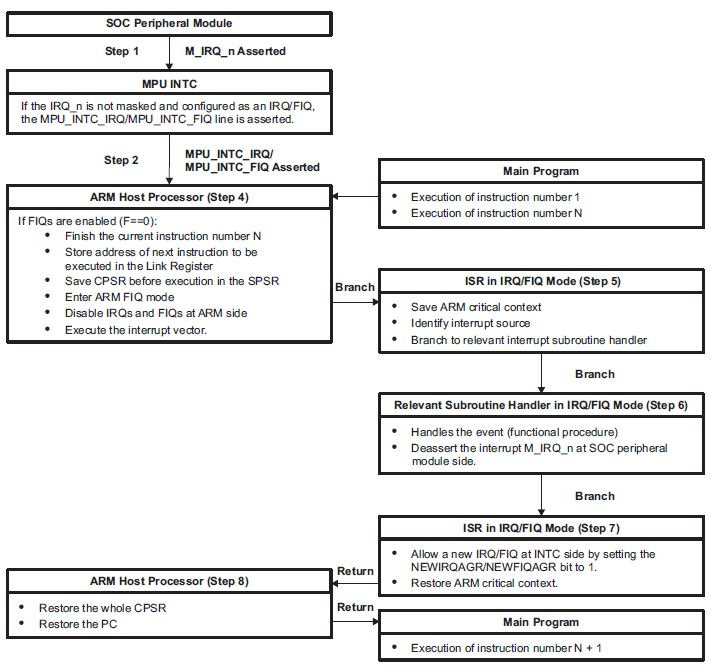
\includegraphics[scale=1]{chapters/hal/figures/interruptProcedure}
	\caption{IRQ/FIQ Verarbeitung \cite[S. 193]{ARM:TRM}}
	\label{fig:interruptProcedure}
\end{figure}


Die Verarbeitung eines Interrupts im Betriebssystem ist in Abbildung \ref{fig:interruptProcessing} schematisch dargestellt. Sichern und Wiederherstellen des aktuellen Kontexts wird durch den in Assembler geschriebenen \textit{IRQ-Handler} vorgenommen. Dieser ruft nach dem Sichern des Kontexts die dem Interrupt zugewiesene Handler-Funktion auf. Nach Behandlung des Interrupts findet eine Wiederherstellung des Kontexts statt, wobei der ursprüngliche Kontext durch die aufgerufene Handler-Funktion durchaus ersetzt oder geändert werden kann.

\begin{figure}[H]
	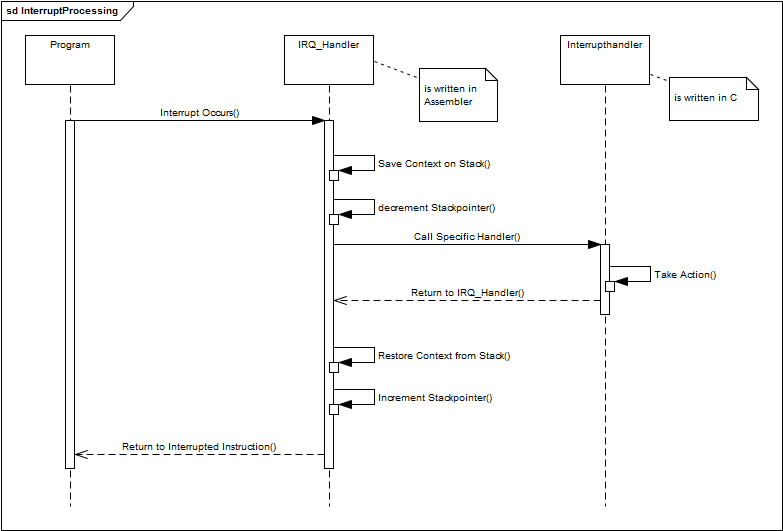
\includegraphics[scale=0.55]{chapters/hal/figures/InterruptProcessing}
	\caption{Interruptverarbeitung im Betriebssystem}
	\label{fig:interruptProcessing}
\end{figure}
\pagebreak 